\documentclass[a4paper, 11pt]{article}
\usepackage{graphicx}
\usepackage[margin=0.78in]{geometry}

\title { Visual Analytics\\ \bigskip \large Propostal: Mobile applications}
\date{21 April 2020}
\author{Silvio Dei Giudici 1708962 \\ Marco Morella 1693765}

\begin{document}

\maketitle

\section{General Idea}
The increasingly cheap mobile technology has induced in the latest years an exponential growth in the mobile application market, to the point that any user has a selection of applications and tools available to download which is so wide and confusing that picking out the fittest one is often a challenge.\\
Due to the particular nature of this problem, the standard app store is often not helpful thus we aim to create a visualization tool where the user can analyze the information given by the store and filter out applications to find the best one dinamically.\\
We will use a dataset containing ten thousand application with all possible information given by the play store, retrieved by web-scraping the browser of Google Play Store, made by an user on kaggle.com.\\
\section{Dataset}
As we said before the dataset contains 10 000 applications, with 13 features which will be analyzed in the following.
\begin{itemize}
\item \textbf{Application name}.
\item \textbf{Category}: one between 34 possible categories in which the Play Store divides its applications, some of which are Game, Business, Communication and so on.
\item \textbf{Rating}: value between 1.0 and 5.0, based on the average review received by the app.
\item \textbf{Reviews}: number of reviews received by the app.
\item \textbf{Size}: size of the app.
\item \textbf{Installs}: number of times the app has been installed by users.
\item \textbf{Type}: whether of not the app is a paid or free one.
\item \textbf{Price}: self-explaining, does not include in-app purchase.
\item \textbf{Content rating}: age group the app is targeted for.
\item \textbf{Genres}: list of genres the app belongs to, e.g. Health, Tools, Entertainment and so on, at this moment we are unsure about how useful this section is and thus we may not use it in the final project.
\item \textbf{Last updated}: date of last update on the play store for the app.
\item \textbf{Android version}: minimum required version to run the application.
\end{itemize}
The database contained one more feature which was deemed not useful for analysis which is \textbf{Current version}. Since every developer uses a different(personal) way to denote the released versions it wouldn't have made much sense in a visualization.\\
In order to be compliant with the AS constraint, since we have 10 000 elements and 11 features we will take less than half of the dataset entries.

\section{MDS}

In this section, we are going to briefly present which are the main choices and ideas for the analysis part of the project and how we want to handle the high cost of computation for the chosen algorithm.   
Indeed, the analysis of the data done by PCA or MDS requires computing power and in general is not possible to do it while the user interacts with the application. 
So in order to make the app usable, we decided to do a preprocessing phase, in which we run the algorithm, and we store the result in the data itself, adding one column for each component. In this way, we run the algorithm only one time and then we load it like a new feature. \\

Another problem that we need to face is which algorithm to use. PCA is often used for these kinds of tasks, but in this case we have more categorical features than continuous values. So we'll probably use MDS because it can be adapted with a lot of kinds of data using a specific distance function. Of course, if we consider only the categorical features than the better choice for a function is the Jaccard distance, but we can do more. Indeed we will try also a different approach with a custom distance function, that considers all the features (both categorical and continuous) merging the Jaccard distance with the euclidian distance and normalizing them, in order to avoid that a type of feature hides the contribution of the other.
%preprocessing
%where to put the coordinates, resulting from the preprocessing script
%mds because there are some categorical feature and also contiguos
%custom distance function, merge with jaccard, euclidian

\section{Visual Project}
In the following we will go over each visualization we want to implement through D3.js, an initial mock-up can be seen in the last page of the proposal.
\begin{itemize}
\item \textbf{Parallel coordinates chart} containing most of the features which should help the user see the general statistic related to the apps he's currenting filtering for.
\item \textbf{Three boxplots} to let the user analyze the distribution over Size, Review and Rate.
\item \textbf{One scatter plot} showing the applications using MDS analysis.
\item \textbf{One horizontal histogram} showing the distribution of samples over the categories.
\item \textbf{One histogram} for the distribution of samples over content rating.
\item \textbf{One histogram} over the occurences of minimum android version required. In order to have a clearer vision of the distribution without having too many separate sections we stacked the different updates of the main version: all y.x stay in the column of y.0.
\end{itemize}
Furthermore we will put a list(or table) of applications fitting in the user filtering. Obviously since this is a proposal made before starting the work we may find out some other visualizations/interaction we may want to implement to improve our visualizations.
\section{User interactions}
In our visualization the user will be able to select one or more value from each parallel coordintes chart to put them in the filter, anything not coherent with those values will be filtered out of the dataset thus reflecting on all other visualizations.\\
The same thing will be doable on all three histograms if any of the column is clicked, else if it the user only hovers over them they will be highlighted on the other graphs.\\
The only items which won't be interactable for the user will be the MDS scatter plot and the boxplots and they will only reflect the changes created by interacting with the previously defined visualizations. \\
We are still discussing wheter or not to add a filter over the Scatter plot to let the user select an item or clusters.
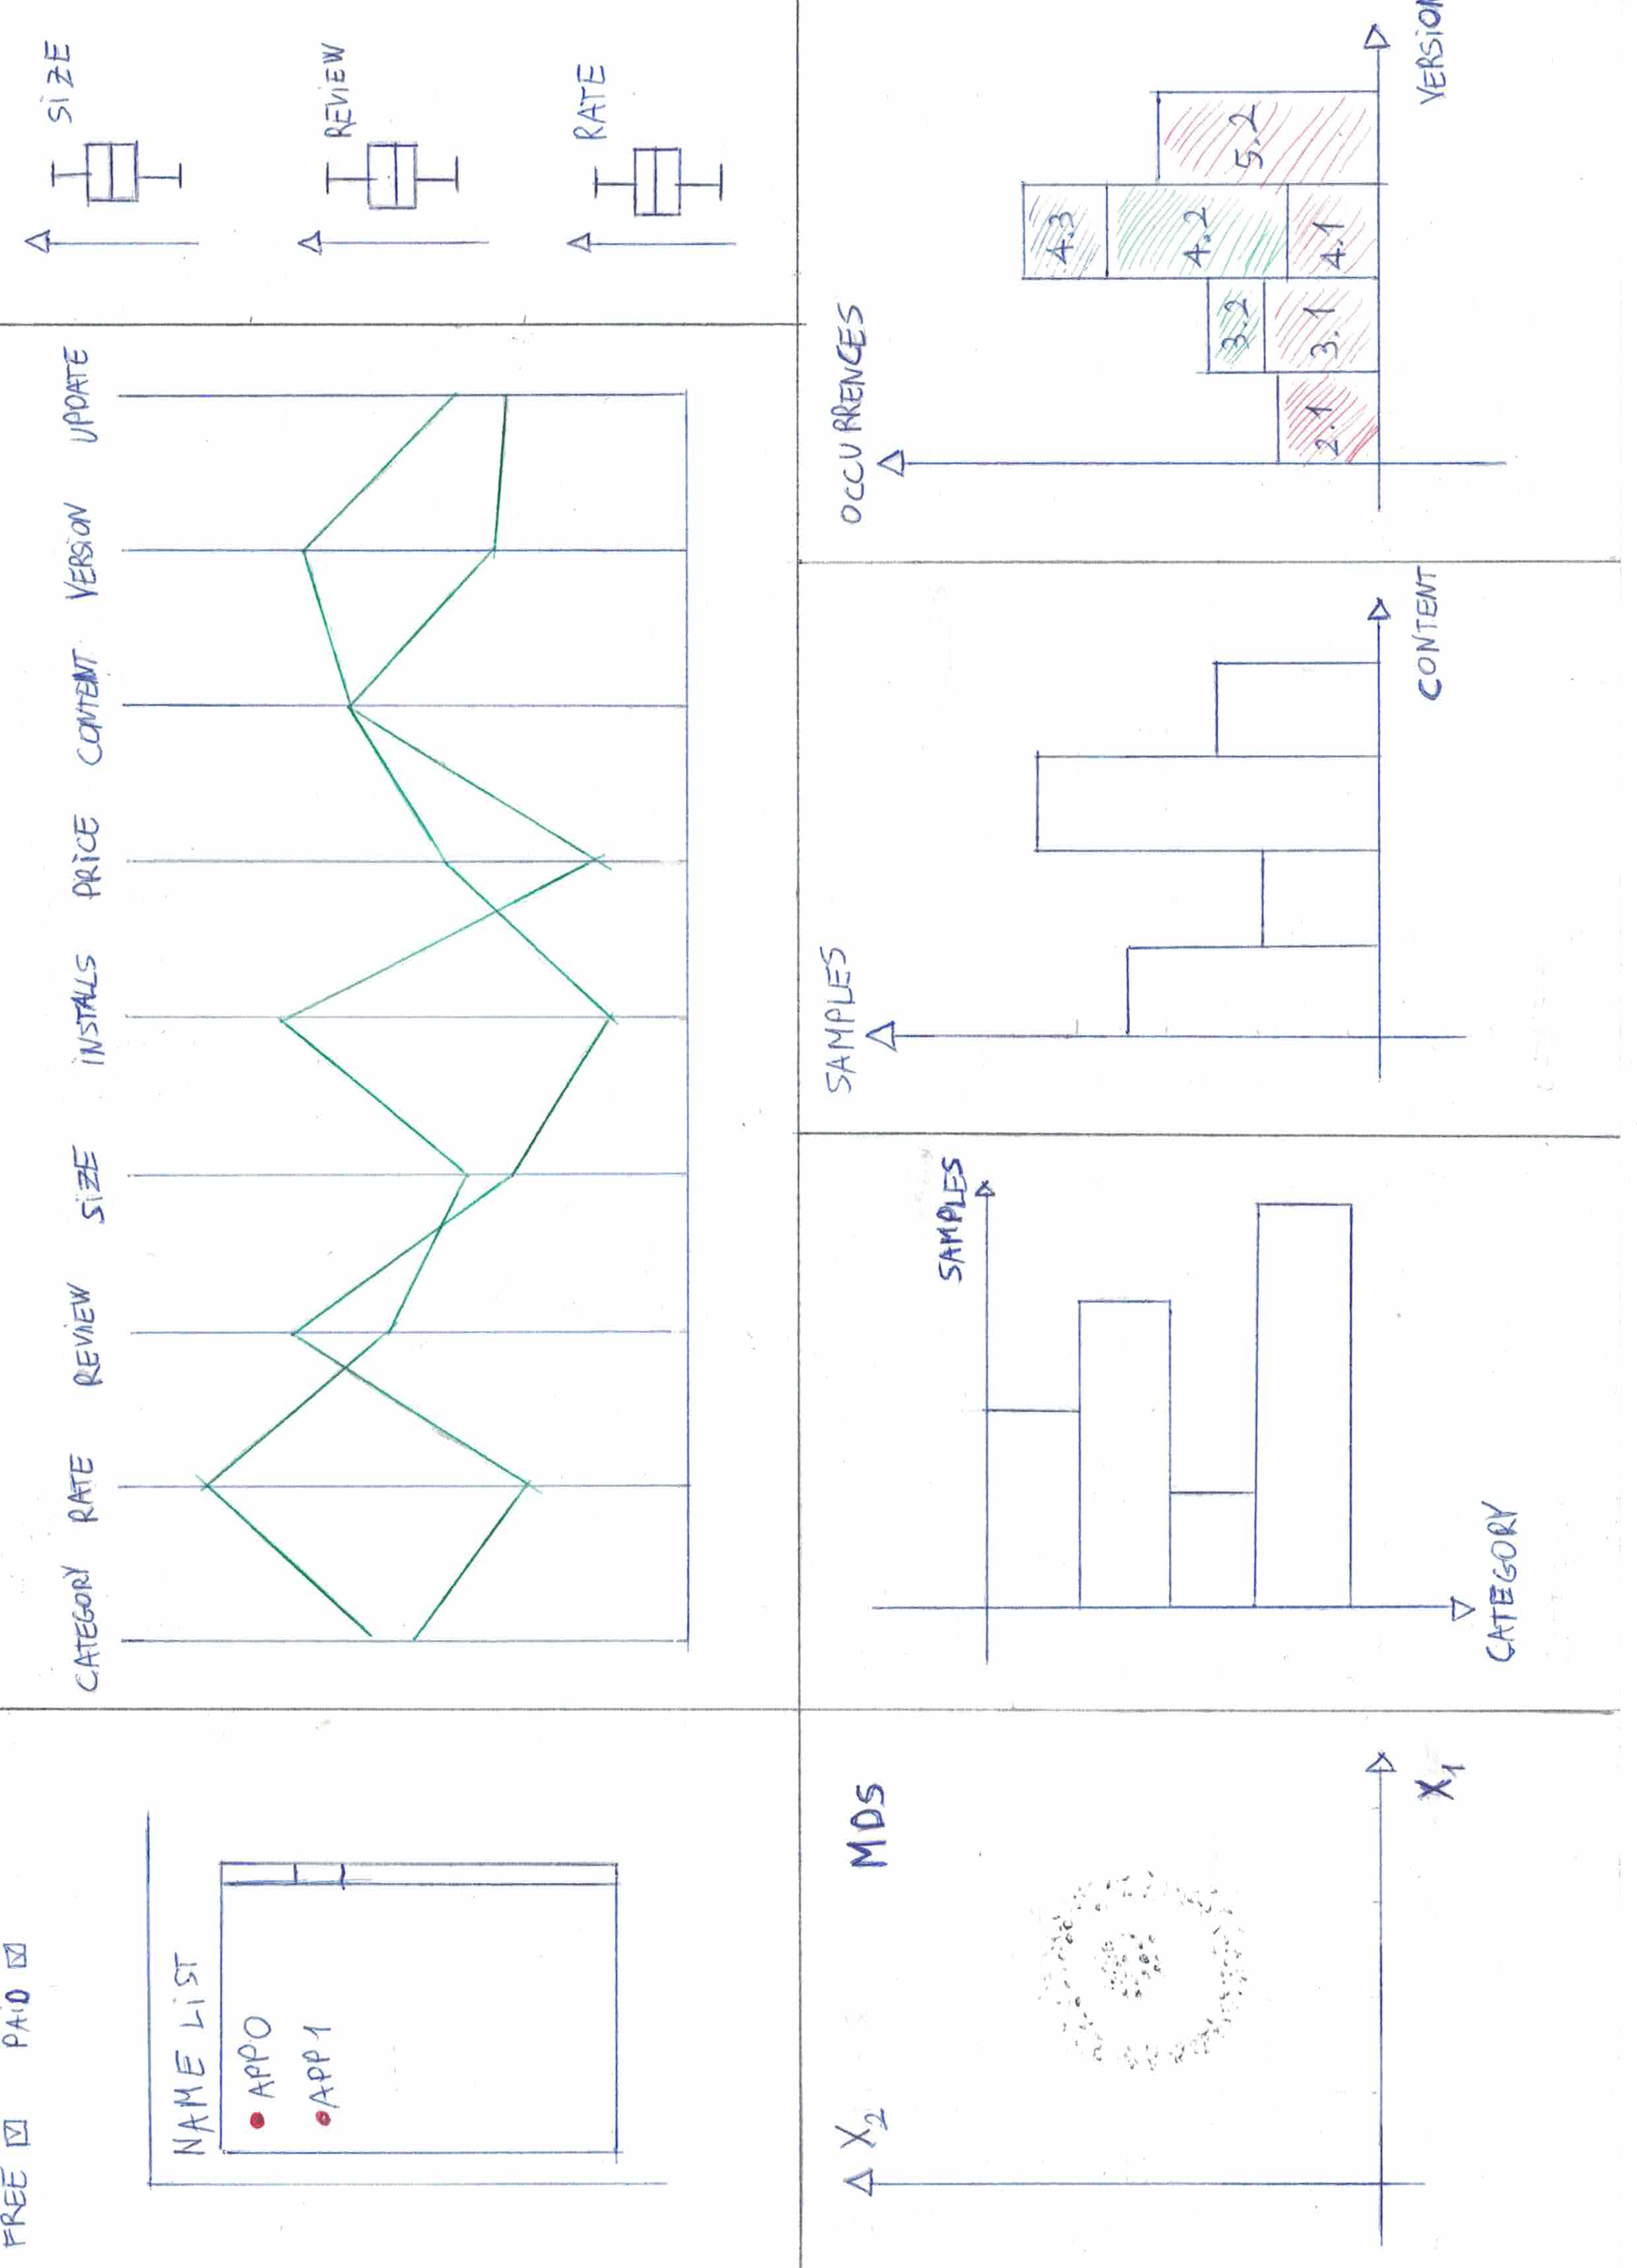
\includegraphics[width=\textwidth, angle=180]{mockup.png}
\end{document}
